\documentclass{article}

\usepackage{calc}
\usepackage{graphicx}
\usepackage{amsmath}
\usepackage{amssymb}
\usepackage{relsize}
\usepackage{multirow}
\usepackage{rotating}
\usepackage{bm}
\usepackage{url}
\usepackage{tikz}
\usepackage{caption}
\usepackage{lipsum}
\usepackage{listings}
\usepackage{graphicx}
\usepackage{multicol}
\usepackage{listings}
\usepackage{graphicx}
\usepackage{multicol}

\usetikzlibrary{calc}
\usetikzlibrary{shapes,arrows,shadows}
\usetikzlibrary{chains,decorations.pathmorphing,positioning,fit}
\usetikzlibrary{decorations.shapes,calc,backgrounds}
\usetikzlibrary{decorations.text,matrix}
\usetikzlibrary{calc}
\usetikzlibrary{mindmap}
\usetikzlibrary{fadings}
\usetikzlibrary{positioning}

% Define some colors:
\definecolor{DarkFern}{HTML}{407428}
\definecolor{DarkCharcoal}{HTML}{4D4944}
\colorlet{Fern}{DarkFern!85!white}
\colorlet{Charcoal}{DarkCharcoal!85!white}
\colorlet{LightCharcoal}{Charcoal!50!white}
\colorlet{AlertColor}{orange!80!black}
\colorlet{DarkRed}{red!70!black}
\colorlet{DarkBlue}{blue!70!black}
\colorlet{DarkGreen}{green!70!black}

\definecolor{lightblue}{rgb}{0.145,0.6666,1}
% set tikz objects
\tikzstyle{textblock} = [rectangle, draw, fill=white!90!Fern, draw=gray!50!yellow, very thick,
    text width=5em, minimum height=2em, align=center]
\tikzstyle{codeblock} = [rectangle, draw, fill=white!90!yellow, draw=gray!50!yellow, very thick,
    text width=2em, minimum height=3em]
\tikzstyle{block} = [rectangle, draw, fill=white, very thick, draw=black,
 rounded corners, minimum height=2em] % fill was DarkFern!30
\tikzstyle{line} = [draw, -latex']
\tikzstyle{cloud} = [draw, ellipse,fill=red!20, node distance=3cm,
    minimum height=2em]

\tikzstyle{myarrows}=[line width=1mm,draw=blue,-triangle 45,postaction={draw, line width=3mm, shorten >=4mm, -}]
\tikzstyle{the_arrow} = [-latex,line width=2mm, draw=blue, blue]


\begin{document}
\pagenumbering{gobble}
%\definecolor{lightblue}{cmyk}{0.83,0.24,0,0.12}
\definecolor{lightblue}{rgb}{0.145,0.6666,1}
\definecolor{airforceblue}{rgb}{0.36, 0.54, 0.66}


%% \begin{tikzpicture}[node distance = 0cm, auto, text width = 7em]
%% %% \begin{center}

%% \node[block, fill=lightblue, minimum height = 5em](expr){
%% \begin{center}  \textbf{Expression} \end{center} };

%% \node[block, right = 3cm of expr, fill=red, minimum height = 20em](gt){
%% \begin{center} \noindent\rule{\linewidth}{1pt}
%%   \noindent\rule{\linewidth}{1pt}
%%   \noindent\rule{\linewidth}{1pt}
%%   \noindent\rule{\linewidth}{1pt}
%%   \noindent\rule{\linewidth}{1pt}
%%   \noindent\rule{\linewidth}{1pt}
%%   \noindent\rule{\linewidth}{1pt}
%%   \noindent\rule{\linewidth}{1pt}
%%   \noindent\rule{\linewidth}{1pt}
%%   \noindent\rule{\linewidth}{1pt}
%%   \noindent\rule{\linewidth}{1pt}
%%   \noindent\rule{\linewidth}{1pt}
%%   \noindent\rule{\linewidth}{1pt}
%%   \noindent\rule{\linewidth}{1pt}
%%   \noindent\rule{\linewidth}{1pt}
%%   \noindent\rule{\linewidth}{1pt}
%%   \noindent\rule{\linewidth}{1pt}
%%   \noindent\rule{\linewidth}{1pt} \end{center}};

%% \node[above = of expr, text width = 8em]{ samples (1e3) $\rightarrow$};
%% \node[left = of expr,  text width = 6em]{ genes (2e4) $\downarrow$};

%% \node[above = of gt, text width = 8em]{ samples (1e3) $\rightarrow$};
%% \node[left = of gt,  text width = 6em]{ SNPs (4e7) $\downarrow$};

%% %% \end{center}
%% \end{tikzpicture}





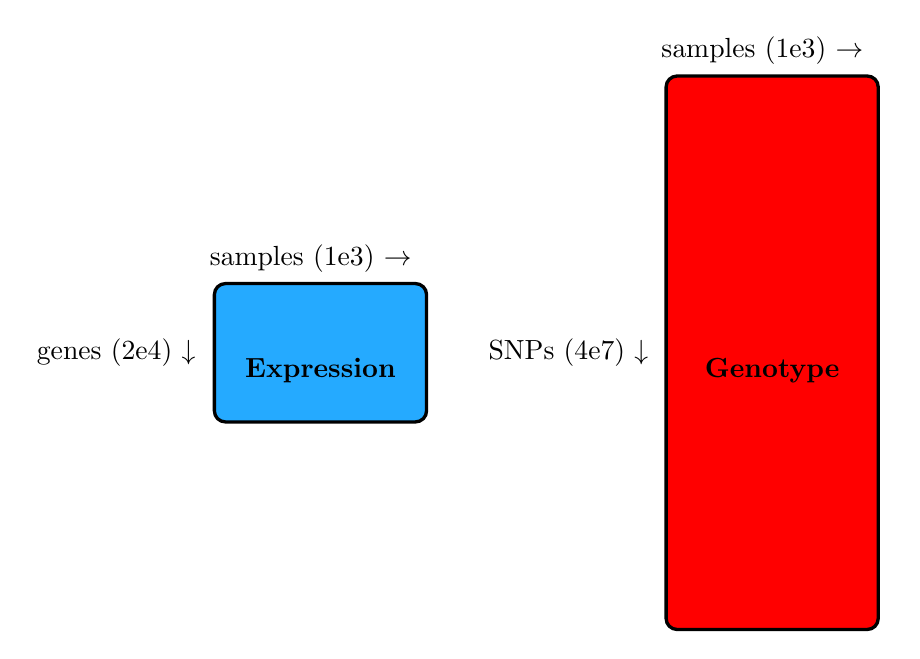
\begin{tikzpicture}[node distance = 0cm, auto, text width = 7em]


\node[block, fill=lightblue, minimum height = 5em](expr){
\begin{center}  \textbf{Expression} \end{center} };

\node[block, right = 3cm of expr, fill=red, minimum height = 20em](gt){
\begin{center} \textbf{Genotype} \end{center}};

\node[above = of expr, text width = 8em]{ samples (1e3) $\rightarrow$};
\node[left = of expr,  text width = 6em]{ genes (2e4) $\downarrow$};

\node[above = of gt, text width = 8em]{ samples (1e3) $\rightarrow$};
\node[left = of gt,  text width = 6em]{ SNPs (4e7) $\downarrow$};

\end{tikzpicture}

\end{document}
